% algorithms: 
% views: 
% containers: adjacency matrix
% data model: incoming edges on a vertex

%% \chapter{Introduction}
%% \label{ch:introduction}

\section{Motivation}

The original STL revolutionized the way that C++ programmers could apply algorithms to different kinds of containers, by defining \emph{generic} algorithms, realized via function templates.  
A hierarchy of \emph{iterators} were the mechanism by which algorithms could be made generic with respect to different kinds of containers,
Named requirements specified the valid expressions and associated types that algorithms required of their arguments.  As of C++20, we now have both ranges and concepts, which
provide language-based mechanisms for specifying requirements for generic algorithms.

As powerful as the algorithms in the standard library are, the underlying basis for them is a range (or iterator pair), which inherently can only specify a one-dimensional container.  
Iterator pairs (equiv.\ ranges) specify a \lstinline{begin()} and an \lstinline{end()} and can move between those two limits in various ways, depending on the type of iterator.
As a result, important classes of problems that programmers are regularly faced with use structures that are not one-dimensional containers, and so the standard library algorithms can't be directly used.
Multi-dimensional arrays are an example of one such kind of data structure. Matrices do have the nice property that they (typically) have the ability to be ``raveled'', i.e., the data underlying the matrix can still be treated as a one-dimensional container.  Multi-dimensional arrays also have the property that, even though they can be thought of as hierarchical containers, the hierarchy is uniform---an N-dimensional array is a container of N-1 dimensional arrays.

Another important problem domain that does not fit into the category of one-dimensional ranges is that of \emph{graph algorithms and data structures}.
Graphs are a powerful abstraction for modeling relationships between entities in a given problem domain,
irrespective of what the actual entities are, and irrespective of what the actual relationships are.
In that sense, graphs are, by their very nature, generic.
Graphs are a fundamental abstraction in computer science, and are ubiquitous in real-world applications.

Any problem concerned with connectivity can be modeled as a graph.  
Just a small set of examples include
Internet routing, circuit partitioning and layout, and finding the best route to take to a destination on map.
There are also relationships between entities that are inferred from large sets of data, for example the graph of consumers who have purchased the same product, or who have viewed the same movie.
Yet more interesting structures (hypergraphs or k-partite graphs) can arise when we want to model relationships between diverse types of data, such as the graph of consumers, the products they have purchased, and the vendors of the products.
And, of course, graphs play a critical role in multiple aspects of machine learning.

Along with these graph abstractions are the graph algorithms that are widely used for sovling problems from these domains.
Well-known graph algorithms include breadth-first search, Dijkstra's algorithm, connected components, and so on.
%
Because graphs can come from so many different problem domains, they will also be represented with many different kinds of data structures.
To make graph algorithms as usable as possible across arbitrary representations requires application of the same principles that were used in the original STL: 
a collection of related algorithms from a problem domain (in our case, graphs),
minimizing the requirements imposed by the algorithms on their arguments,
systematically organizing the requirements, and
realizing this framework of requirements in the form of concepts.

There are also many uses of graphs that would not be met by a standard set of algorithms.  A standardized interface for graphs is eminently useful in such situations as well.  
In the most basic case, it would provide a well-defined framework for development.  But in keeping with the foundational goal of generic programming to enable reuse, it would also empower users to develop and deploy their own reusable graph components.  In the best case, such algorithms would be available to the broader C++ programmer community.

Because graphs are so ubiquitous and so important to modern software systems, a standardized library of graph algorithms and data structures would have enormous benefit to the C++ development community.
This proposal contains the specification of such a library, developed using the principles above.



\section{Example: Six Degrees of Kevin Bacon}
\label{sec:bacon}

A classic example of the use of a graph algorithm is the game ``The Six Degrees of Kevin Bacon.''
The game is played by connecting actors to each other through movies they have appeared in together.
The goal is to find the smallest number of movies that connect a given actor to Kevin Bacon.
That number is called the ``Bacon number'' of the actor. Kevin Bacon himself has a Bacon number of 0.
Since Kevin Bacon appeared with Tom Cruise in ``A Few Good Men'', Tom Cruise has a Bacon number of 1.

The following program computes the Bacon number for a small selection of actors.

% \phil{Duplicated in Overview's Examples. OK?}
{\small
  \lstinputlisting[firstline=26,lastline=48]{D3126_Overview/src/bacon.cpp}
}


\noindent
Output:
\begin{lstlisting}
Tom Cruise has Bacon number 1
Kevin Bacon has Bacon number 0
Hugo Weaving has Bacon number 3
Carrie-Anne Moss has Bacon number 4
Natalie Portman has Bacon number 2
Jack Nicholson has Bacon number 1
Kelly McGillis has Bacon number 2
Harrison Ford has Bacon number 1
Sebastian Stan has Bacon number 3
Mila Kunis has Bacon number 3
Michelle Pfeiffer has Bacon number 1
Keanu Reeves has Bacon number 4
Julia Roberts has Bacon number 1    
\end{lstlisting}  


In graph parlance, we are creating a graph where the vertices are actors and the edges are movies.
The number of movies that connect an actor to Kevin Bacon is the shortest path in the graph
from Kevin Bacon to that actor. In the example above, we compute shortest paths from Kevin
Bacon to all other actors and print the results.
Note, however, that actor-actor relationships are not how data about actors
is available in the wild (from IMDB, for example).  Rather, two available types of data are actor-movie and movie-actor relationships.  See Section~\ref{sec:bipartite} below.


\section{Graph Background} %  and Terminology}

For clarity, we briefly review some of the basic terminology of graphs.
We use commonly accepted terminology for graph data structures and algorithms and
adopt the particular terminology used in the textbook by
Cormen, Leiserson, Rivest, and Stein (``CLRS'')~\cite{CLRS2022}.
%
In defining terminology that is rich enough, yet precise enough, to be used as the basis of a C++ graph library, we emphasize the difference between a graph (an abstraction of entities in a domain, along with their relationships) and the \emph{representation} of a graph (a structure suitable for use by algorithms and/or for code)\footnote{An example of the kind of ambiguity about graphs arising in typical usage is shown in Appendix~\ref{sec:ambiguity}}.
% We note that because of the precision with which we define representations, there will be some unexpected results.

\section{Summary of Key Takeaways}
A very brief summary of our terminology is the following:
\begin{itemize}
  \item A graph comprises a set of vertices $\{V\}$ and a set of edges $\{E\}$, written $G=\{V, E\}$.
  \item Expressing algorithms (mathematically as well as in code) requires a \emph{representation} of a graph, the most basic of which is an \emph{adjacency matrix}.  An adjacency matrix is constructed using an \emph{enumeration} of the vertices, not the vertices themselves.
    \item In addition to the (dense) adjacency matrix representation, we consider three sparse representations: coordinate, compressed, and packed coordinate.  The sparse forms store \emph{indices} used in the enumeration.
    \item The coordinate and compressed forms of the adjacency matrix, as taken from linear algebra, respectively correspond to the graph theoretical representations of \emph{edge list} and \emph{adjacency list}.
\end{itemize}


\subsection{Basic Terminology}

To model the relationships between entities, a \emph{graph} $G$ comprises two sets:
a \emph{vertex set} $V$, whose elements correspond to the entities, and an \emph{edge set} $E$, whose
elements are pairs corresponding to elements in $V$ that have some relationship with each other.  That is,
if $u$ and $v$ are members of $V$ that have some relationship that we wish to capture, then there is
a pair $\{u, v\}$ in $E$.  We write $G=\{V, E\}$ to express that the two sets $V$ and $E$ define a graph $G$.

Figures~\ref{subfig:airport} and~\ref{subfig:instagram} show two examples of graph models,
a network of airline routes between cities and a social network of names and followers.
The figures indicate the domain-specific data to be modeled and the sets $V$ and $E$ for each graph.
Each figure also includes a node and link diagram, a commonly-used graphical\footnote{An unfortunate collision of terminology.}
notation.

\begin{figure}[ht]
  \begin{center}
    \subcaptionbox{An undirected graph representing airline routes between cities.  Shown are the list of airports (the vertices) and the list of routes between them (the  edges).  Also shown are a node and link diagram and the set-based description.\label{subfig:airport}}
    {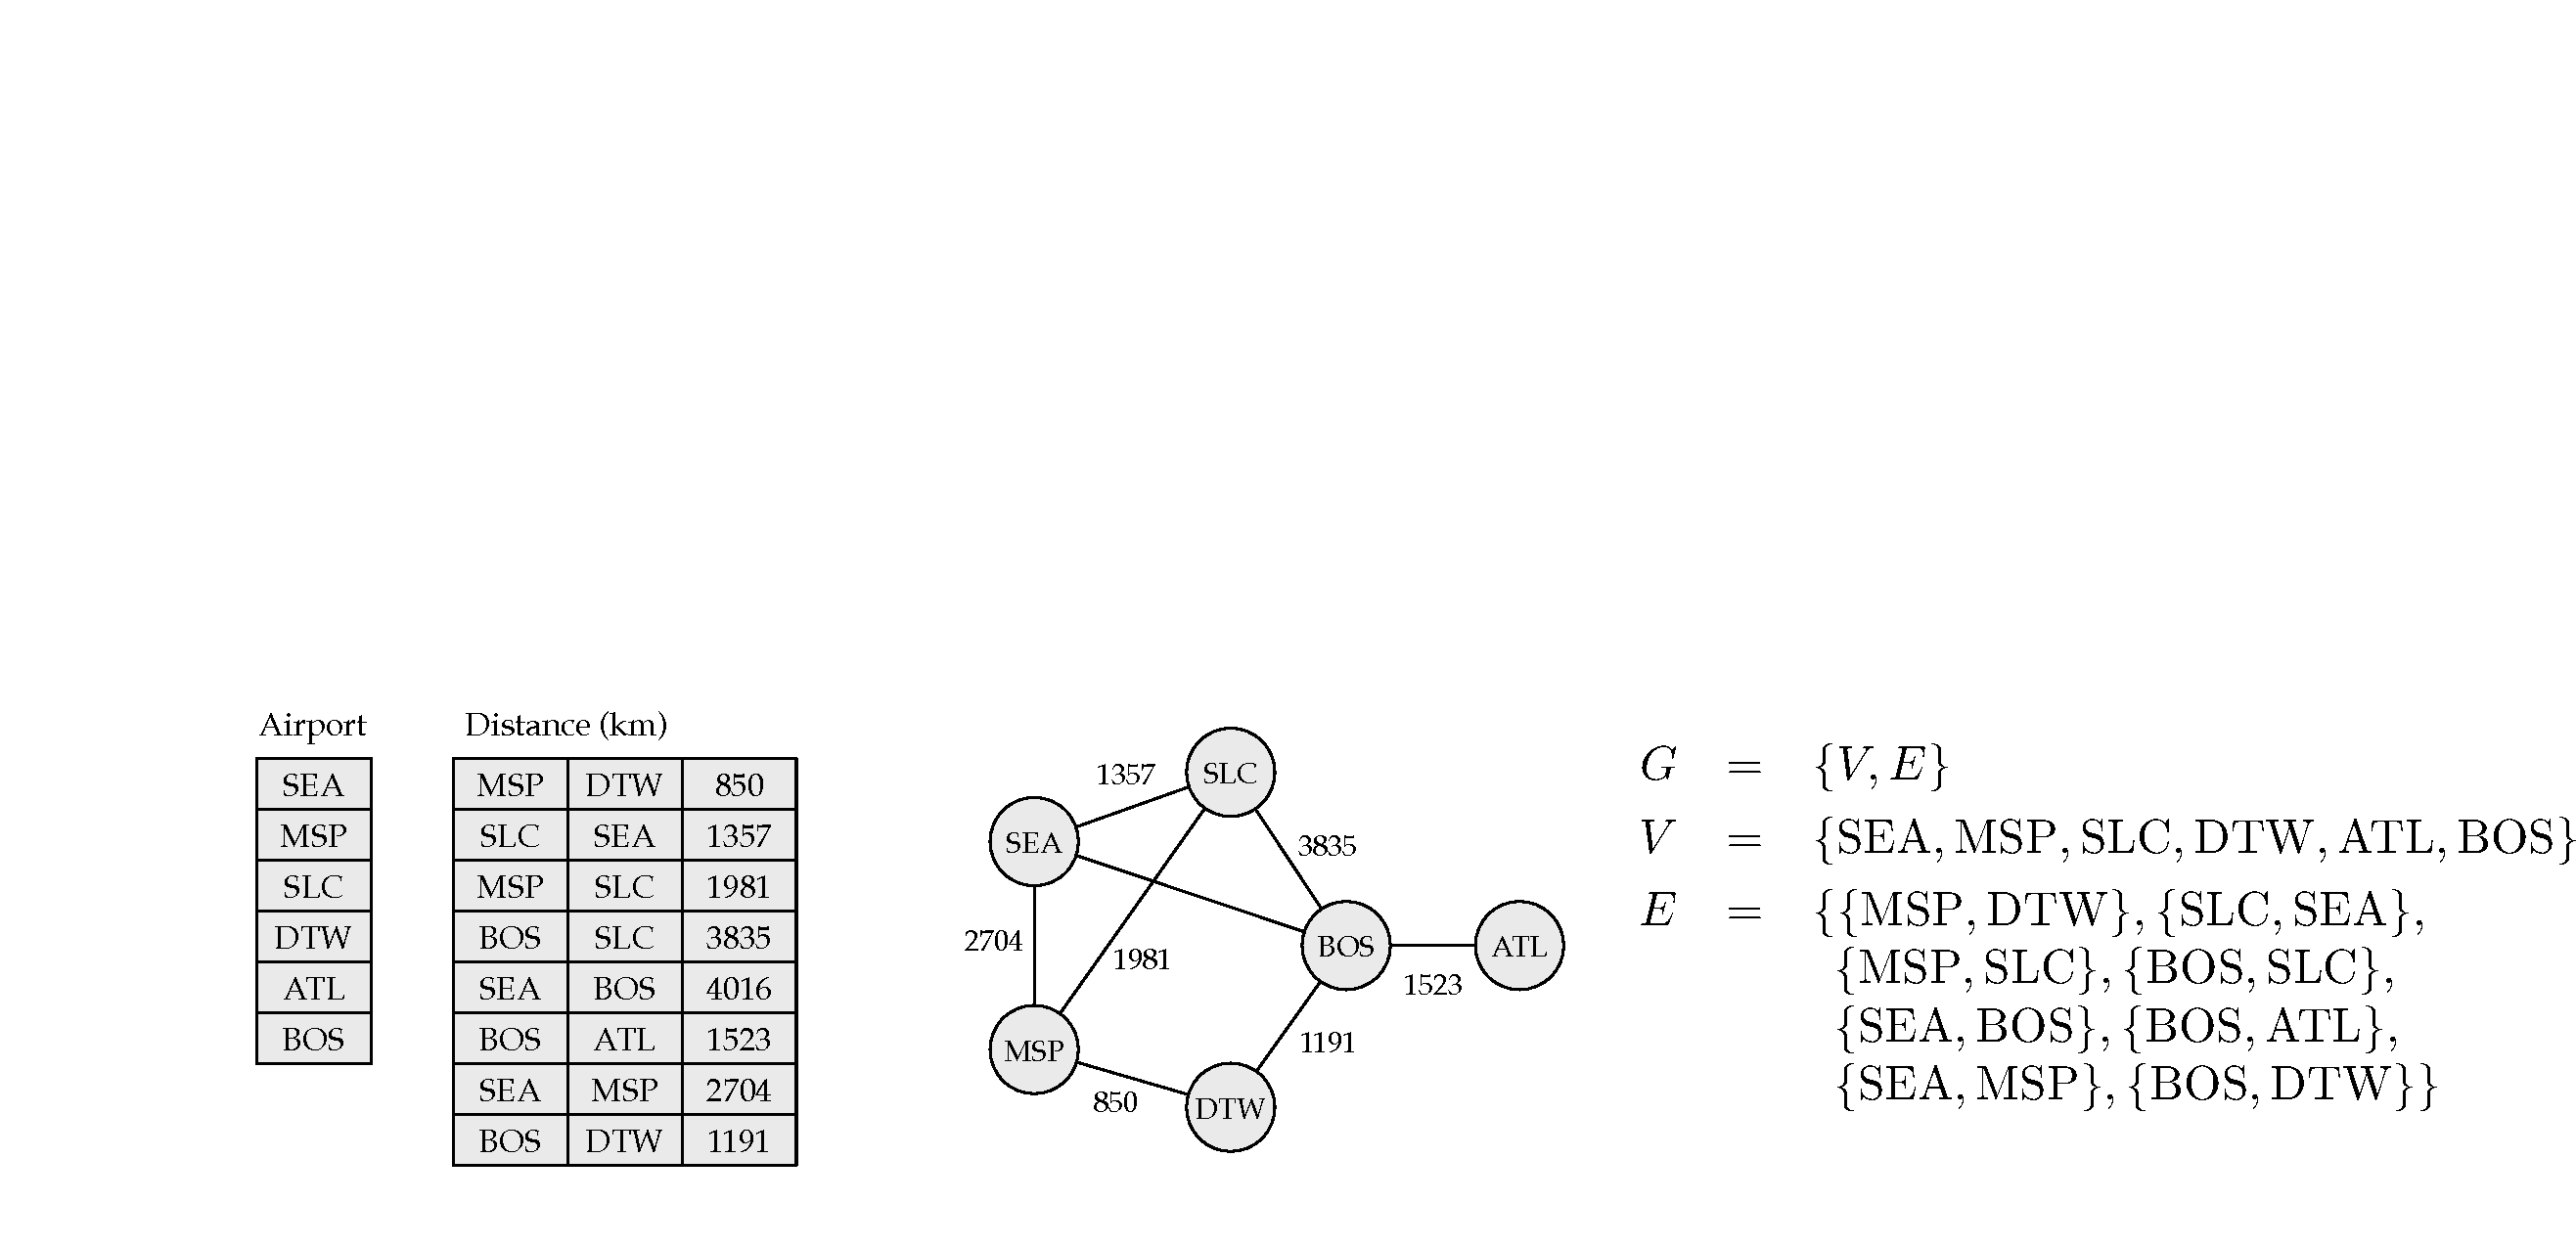
\includegraphics[width=0.75\textwidth]{figs/airport-summary.pdf}}
    \\
    \subcaptionbox{A directed graph representing followers in a social network.  Shown in the diagram are the names of members (the vertices) and the members they follow (the edges). Since following is a one-way relationship, we use a directed graph to model it.  Also shown are a node and link diagram and the set-based description.\label{subfig:instagram}}
    {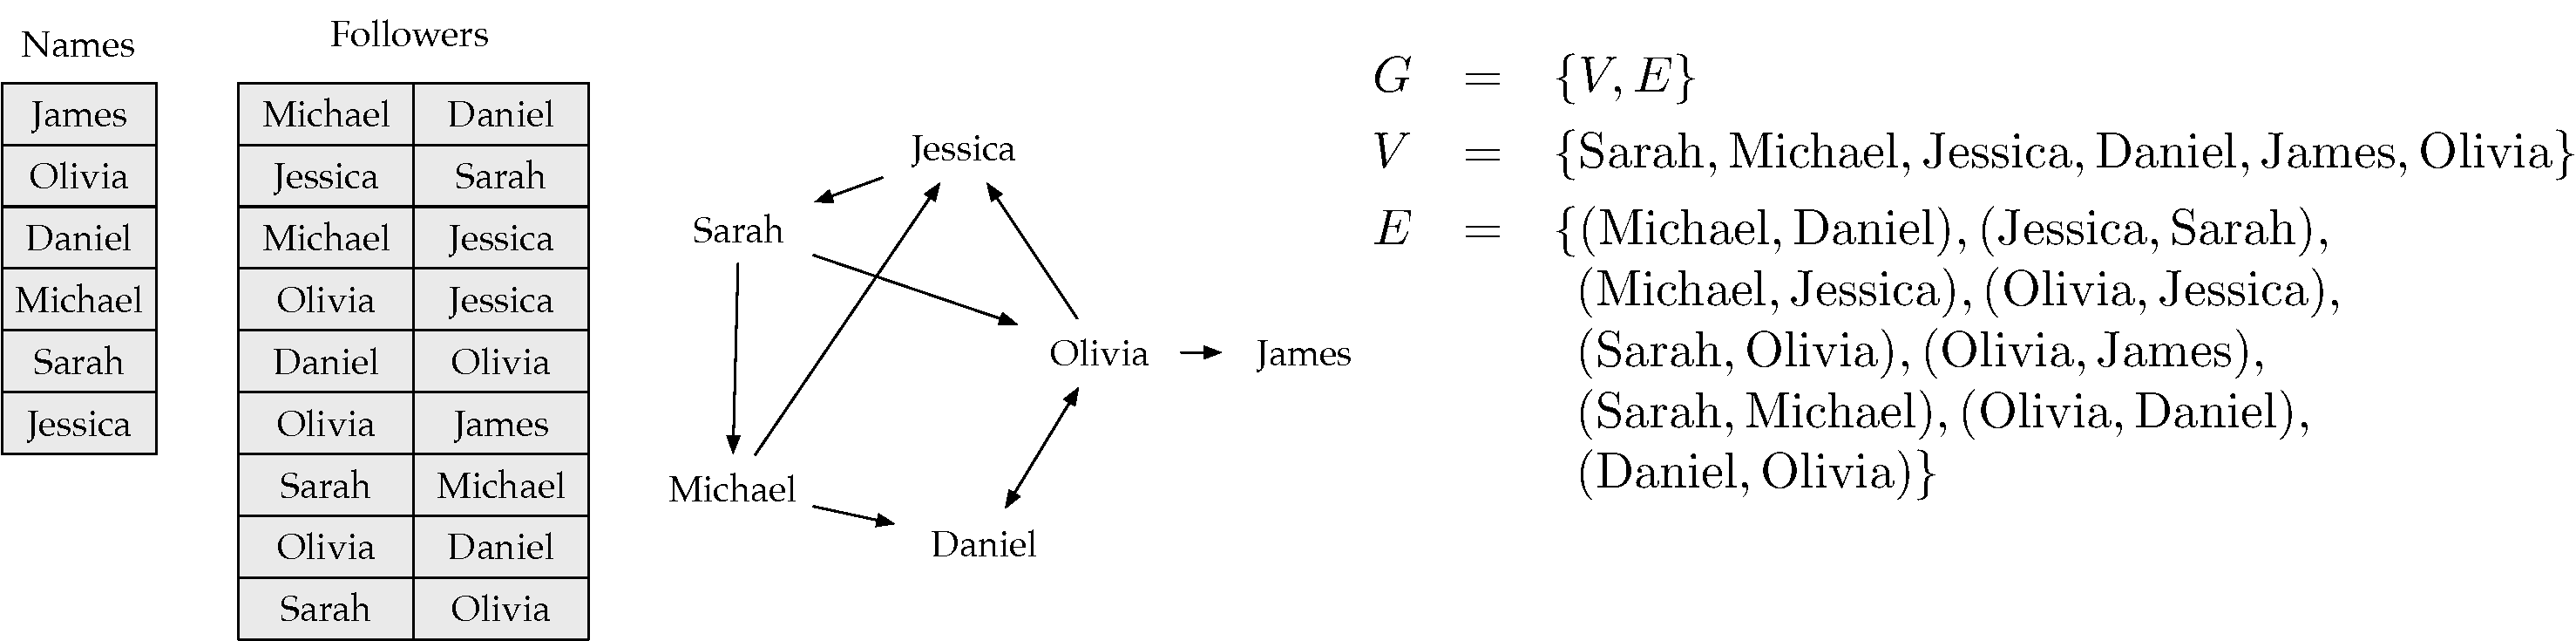
\includegraphics[width=0.825\textwidth]{figs/instagram-summary.pdf}}
    \caption{Graph models of an airline route system and of a social media follower network.\label{fig:node_link_graphs}}
  \end{center}
\end{figure}


\subsection{Graph Representation: Enumerating the Vertices}

To reason about graphs, and to write algorithms for them, we require a concrete \emph{representation} of the graph.
We note that \emph{a graph and its representation are not the same thing}.  It is therefore essential
that we be precise about this distinction as we develop a software library of graph
algorithms and data structures\footnote{In fact, if we are to be completely precise, the library we are
proposing is one of algorithms and data structures for graph representations.  We will make concessions
to commonly accepted terminology, while precisely defining that terminology.}.

The representations that we will be using are familiar ones: adjacency matrix, edge list, and adjacency list.
We begin with a process that is so standard that we typically don't even notice it, but it forms
the foundation of all graph representations: we \emph{enumerate the vertices.}  That is, we assign an
index to each element of $V$ and write $V = \{v_0, v_1, \ldots v_{n-1}\}$.  Based on that enumeration,
elements of $E$ are expressed in the form $\{v_i, v_j\}$.  Similarly, we can enumerate the edges, and write  
$E = \{ e_0, e_1, \ldots e_{m-1}\}$, though the enumeration of $E$ does not play a role in standard
representations of graphs.
%
The number of elements in $V$ is denoted by $|V|$ and the number of elements in $E$ is denoted by $|E|$.

We summarize some remaining terminology about vertices and edges.
\begin{itemize}
\item 
An edge $e_k$ may  be \emph{directed}, denoted as the ordered pair $e_k=(v_i, v_j)$, or it may be
  \emph{undirected}, denoted as the (unordered) set $e_k=\{v_i, v_j\}$.  The edges 
in $E$ are either all directed or all undirected,
  corresponding respectively to a \emph{directed graph} or to an \emph{undirected} graph.
\item 
If the edge set $E$ of a directed graph contains an edge $e_k = (v_i,v_j)$, then
  vertex $v_j$ is said to be \emph{adjacent} to vertex $v_i$.  The edge $e_k$ is an
  \emph{out-edge} of vertex $v_i$ and an in-edge of vertex $v_j$.  Vertex $v_i$ is the \emph{source} of
  edge $e_k$, while $v_j$ is the \emph{target} of edge $e_k$.
\item If the edge set $E$ of an undirected graph contains an edge $e_k = \{v_i,v_j\}$, then
  $e_k$ is said to be \emph{incident} on the vertices $v_i$ and $v_j$.
  Moreover, vertex $v_j$ is adjacent to vertex $v_i$
  \emph{and} vertex $v_i$ is adjacent to vertex $v_j$.
  The edge $e_k$ is an out-edge of both $v_i$ and $v_j$ and it is an in-edge of both $v_i$ and $v_j$.
\item The \emph{neighbors} of a vertex $v_i$ are all the vertices $v_j$ that are adjacent to $v_i$.  The set of all the neighbors of $v_i$ is the \emph{neighborhood} of $v_i$.
\item A \emph{path} is a sequence of vertices $v_0, v_1, \ldots, v_{k-1}$ such that
there is an edge from $v_0$ to $v_1$, an edge from $v_1$ to $v_2$, and so on.
That is, a path is a set of edges $(v_i, v_{i+1}) \in E$ for  $i = 0, 1, \ldots, k-2$.
\end{itemize}


\subsection{Adjacency-Based Representations}

We begin our development of graph representations
with the almost universally-accepted definition of the
adjacency matrix representation of a graph.
%
The \emph{adjacency matrix representation} of a graph $G$ is a $|V|\times |V|$ matrix $A = (a_{ij})$ such that,
respectively for a directed or undirected graph
\[
 a_{i j} = 
 \left\{
 \begin{array}{rl}
  1 & \textrm{if } (v_i, v_j) \in E \\
  0 & \textrm { otherwise }
 \end{array}
 \right.
 \qquad\qquad
 a_{i j} = a_{ji} =
 \left\{
 \begin{array}{rl}
  1 & \textrm{if } (v_i, v_j) \in E \\ 
  0 & \textrm { otherwise }
 \end{array}
 \right.
\]
That is, $a_{ij} = 1$ if and only if $v_j$ is adjacent to $v_i$ in the original graph $G$ (hence the name ``adjacency matrix``).  We note that the difference between the adjacency matrices for a directed vs an undirected graph is that and the adjacency matrix for an undirected graph has $a_{ji} = 1$ whenever $a_ij$ is equal to one.  That is, it is symmetric.

Here we can see also why we said that the initial enumeration of $V$ is foundational to representations:  \emph{The adjacency matrix is based solely on the indices used in that enumeration}.  It does not contain the vertices or edges themselves.  The enumeration corresponding to vertices is implicit: the neighbor information for vertex $v_i$ is stored on row $i$ of the matrix.  Similarly, we don't store an edge $(v_i, v_j)$ explicitly, but rather an indicator as to whether $(v_i, v_j)$ exists in $E$ or not.

As a data structure to use for algorithms, the adjacency matrix is not very efficient, neither in terms of storage (which, at $|V|\times |V|$ is prohibitive), nor for computation, because for many graphs, the adjacency matrix contains almost all zero elements. Instead of storing the entire
adjacency matrix, we can simply store the index values of its non-zero elements.  A \emph{sparse coordinate adjacency
matrix} is a container $C$ of pairs $(i, j)$ for every $a_{ij}$ in $A$.

\textbf{NB:} At first glance, it may seem that we have simply created a data structure $C$ that has a pair $(i,j)$ if $E$ in the
original graph has an edge from $v_i$ to $v_j$.  This is true in the directed case.  However, in the undirected case, if there is an edge between $v_i$ and $v_j$, then $v_i$ is adjacent to $v_j$, and $v_j$ is adjacent to $v_i$.  In other words, if there is an edge between $v_i$ and  $v_j$ in an undirected graph, then both the entries $a_{ij}$ and $a_{ji}$ are equal to $1$\footnote{That is, the adjacency matrix is symmetric.} --- and therefore for a single edge between $v_i$ and $v_j$,  $C$ contains two index pairs: $(i, j)$  and $(j, i)$.   The sparse coordinate representation is commonly known as \emph{edge list}.  However, we caution the reader that $C$ does not store edges, but rather indices that represent adjacencies between vertices.  In the case that $C$ represents an undirected graph, there is not a 1-1 correspondence between the edges in $E$ and the contents of $C$.

Although the sparse coordinate adjacency matrix is much more efficient in terms of storage than the original adjacency matrix, it isn't as efficient as it could be.  
Much more importantly, it is not useful for the types of operations used by most graph algorithms, which need to be able to get the set of neighbors of a given vertex in constant time.  
To support this type of operation, we use a \emph{compressed sparse adjacency matrix}, which is an array $J$ with $|V|$ entries, where each $J[i]$ is a linear container of indices $\{ j \}$ such that $v_j$ is a neighbor of (is adjacent to) $v_i$ in $G$.  
That is $j$ is contained in $J[i]$ if and only if there is an edge $(v_i, v_j)$ in $E$ (or, equivalently, if there is a pair $(i, j)$ in $C$ or, equivalently, if $a_{ij} = 1$)\footnote{The compressed sparse adjacency matrix is identical to the compressed sparse row format from linear algebra}.  
We note that if $(v_i, v_j)$ is an edge in an undirected graph, $J[i]$ will contain $j$ and $J[j]$ will contain $i$. 
The common name for this data structure is \emph{adjacency list}.  
Although this name is problematic (for instance, it is not actually a list),  it is so widely used that we also use it here---but \emph{we mean specifically that an  ``adjacency list'' is the compressed sparse adjacency matrix representation of a graph}\footnote{We concede that ``adjacency list'' rolls off the tongue much more easily than ``compressed sparse adjacency matrix representation of a graph.''}.  
Again we emphasize the distinction between a graph and its representation:  An adjacency list $J$ is not the same as the graph $G$---it is a representation of $G$, based on an enumeration of the vertices in $\{V\}$.

Illustrations of the adjacency-matrix representations of the airline route graph and the electronic instagram graph are shown in Figures~\ref{fig:airport-representation} and~\ref{fig:instagram}, respectively.

\begin{figure}[tbh]
  \begin{subfigure}[t]{0.175\textwidth}
    \centering
    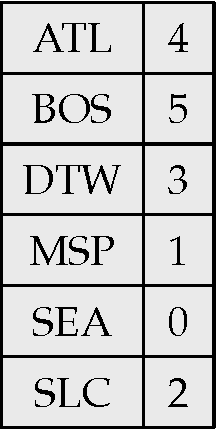
\includegraphics[width=0.4\linewidth]{airport-vertex-enumeration}
    \caption{\label{fig:airport-vertex-enumeration}
    An enumeration of the airport graph given in \protect\ref{subfig:airport}.}
  \end{subfigure}
  \hspace{1em}
  \begin{subfigure}[t]{0.25\textwidth}
    \centering
    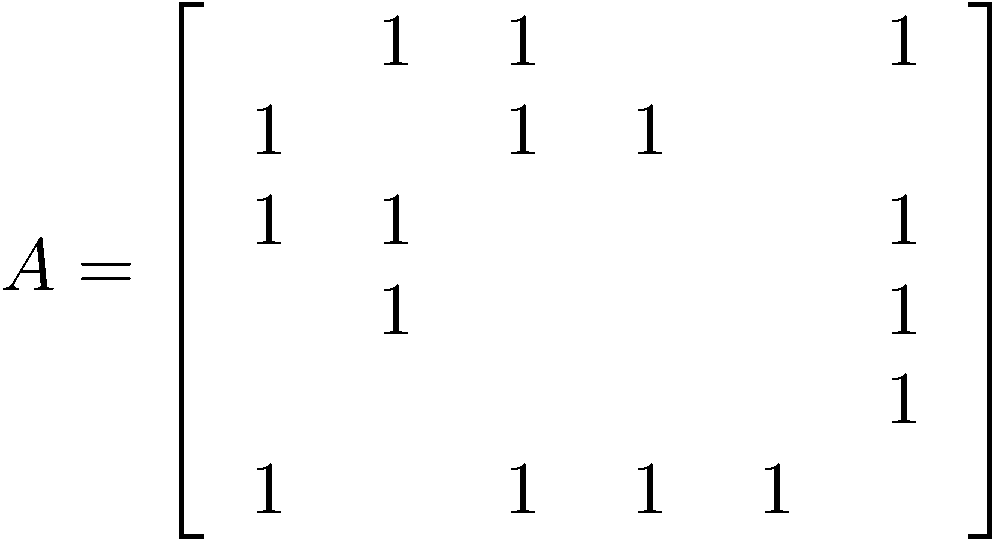
\includegraphics[width=\linewidth]{airport-graph-adjacency-matrix}
    \caption{\label{fig:airport-graph-adjacency-matrix}
    The adjacency matrix representation of the graph given in Figure~\protect\ref{subfig:airport},
    using the enumeration given in Figure~\protect\ref{fig:airport-vertex-enumeration}.}
  \end{subfigure}
  \hspace{1em}
  \begin{subfigure}[t]{0.175\textwidth}
    \small
    \centering
    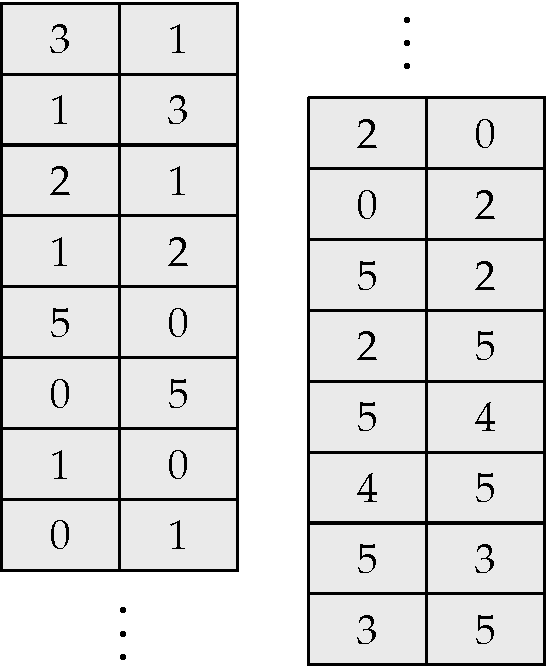
\includegraphics[width=0.7\linewidth]{split-airport-coordinate-sparse-adjacency}
    \caption{\label{fig:airport-coordinate-sparse-adjacency}
    The coordinate sparse adjacency matrix representation (shown split into two columns).}
  \end{subfigure}
  \hspace{1em}
  \begin{subfigure}[t]{0.3\textwidth}
    \small
    \centering
    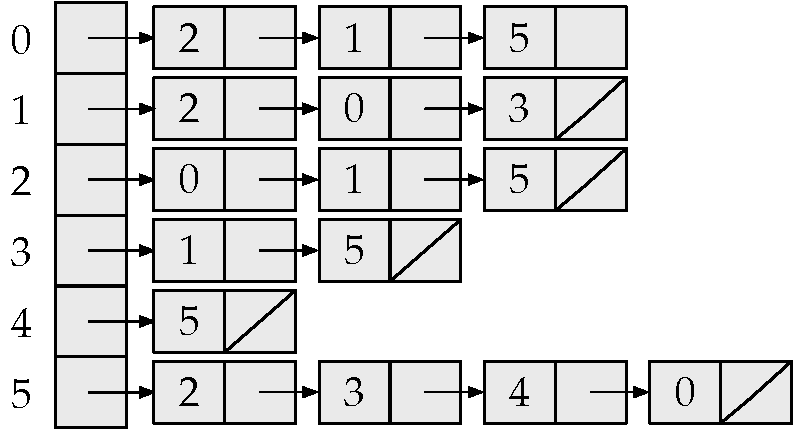
\includegraphics[width=0.75\linewidth]{airport-compressed-sparse-adjacency}
    \caption{\label{fig:airport-compressed-sparse-adjacency}
    The compressed sparse adjacency matrix representation.}
  \end{subfigure}
  \caption{Adjacency matrix representations of the airport graph model.\label{fig:airport-representation}}
\end{figure}



\begin{figure}[tbh]
  \begin{subfigure}[t]{0.175\textwidth}
    \centering
    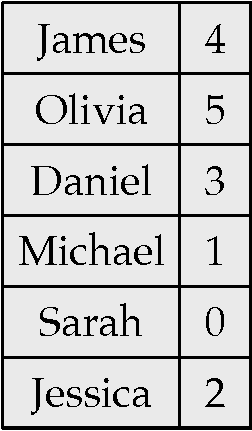
\includegraphics[width=0.4\linewidth]{instagram-vertex-enumeration}
    \caption{\label{fig:instagram-vertex-enumeration}
    An enumeration of the instagram graph given in \protect\ref{subfig:instagram}.}
  \end{subfigure}
  \hspace{1em}
  \begin{subfigure}[t]{0.25\textwidth}
    \centering
    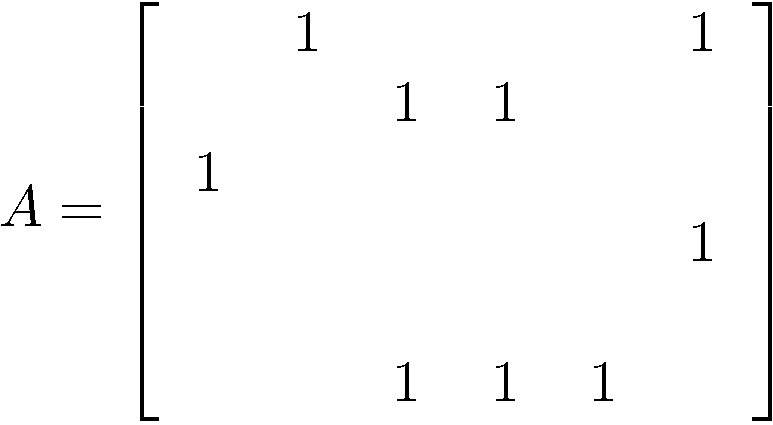
\includegraphics[width=\linewidth]{instagram-graph-adjacency-matrix}
    \caption{\label{fig:instagram-graph-adjacency-matrix}
    The adjacency matrix representation of the graph given in Figure~\protect\ref{subfig:instagram},
    using the enumeration given in Figure~\protect\ref{fig:instagram-vertex-enumeration}.}
  \end{subfigure}
  \hspace{1em}
  \begin{subfigure}[t]{0.175\textwidth}
    \small
    \centering
    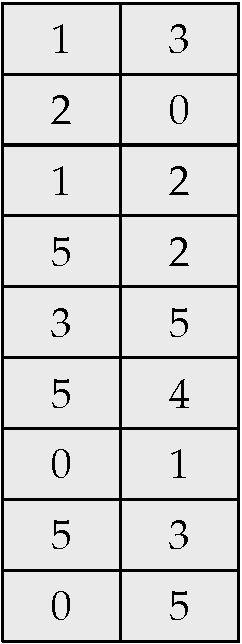
\includegraphics[width=0.4\linewidth]{instagram-coordinate-sparse-adjacency}
    \caption{\label{fig:instagram-coordinate-sparse-adjacency}
    The coordinate sparse adjacency matrix representation.}
  \end{subfigure}
  \hspace{1em}
  \begin{subfigure}[t]{0.3\textwidth}
    \small
    \centering
    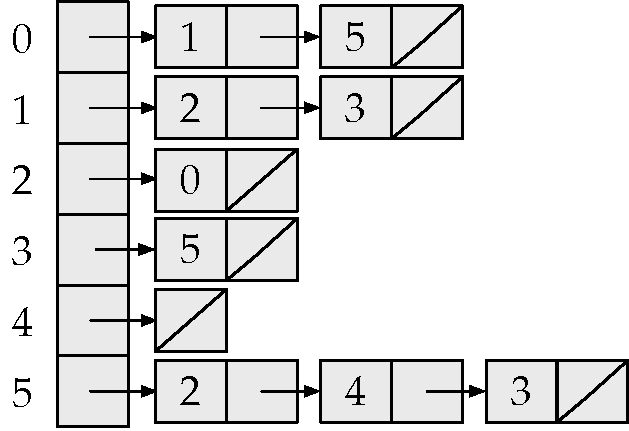
\includegraphics[width=0.75\linewidth]{instagram-compressed-sparse-adjacency}
    \caption{\label{fig:instagram-compressed-sparse-adjacency}
    The compressed sparse adjacency matrix representation.}
  \end{subfigure}
  \caption{Adjacency matrix representations of the instagram graph model.\label{fig:instagram}}
\end{figure}


\section{Bipartite Graphs}
\label{sec:bipartite}

\begin{figure}[ht]
 \begin{subfigure}[t]{0.15\textwidth}
    \small
    \centering
    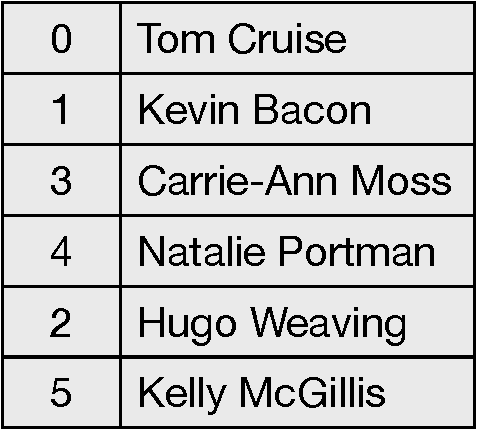
\includegraphics[width=0.825\linewidth]{figs/actor-table.pdf}
    \caption{\label{fig:actor-table}
    Table of actors.}
  \end{subfigure}
\hspace{1em}
   \begin{subfigure}[t]{0.167\textwidth}
    \small
    \centering
    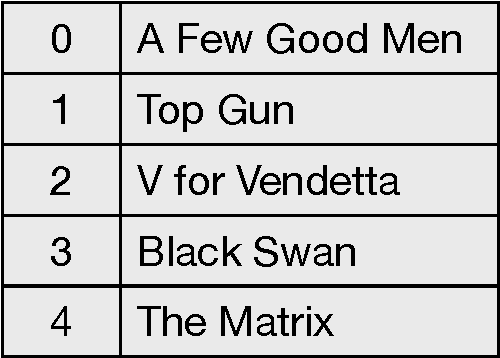
\includegraphics[width=0.825\linewidth]{figs/movie-table.pdf}
    \caption{\label{fig:movie-table}
    Table of movies.}
  \end{subfigure}
\hspace{1em}
     \begin{subfigure}[t]{0.3\textwidth}
    \small
    \centering
    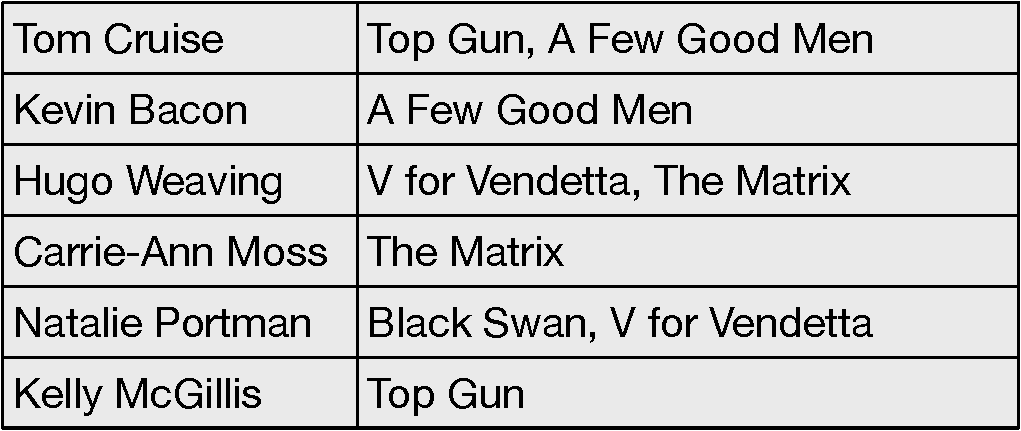
\includegraphics[width=0.825\linewidth]{figs/actor-movie-table.pdf}
    \caption{\label{fig:actor-movie-table}
    A table of actors and movies they have appeared in.}
  \end{subfigure}
\hspace{1em}
       \begin{subfigure}[t]{0.3\textwidth}
    \small
    \centering
    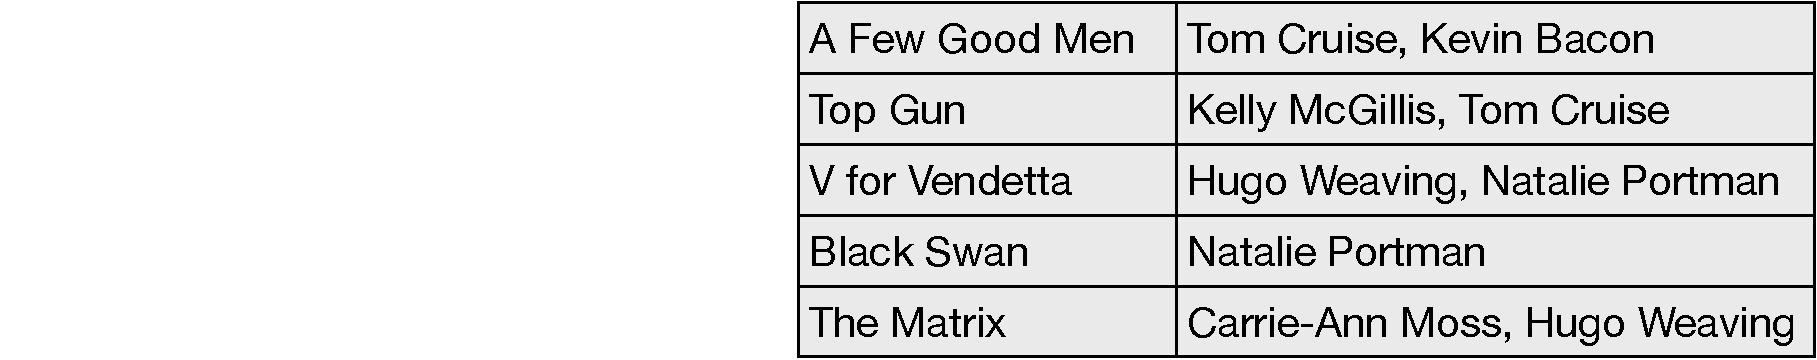
\includegraphics[width=0.9\linewidth]{figs/movie-actor-table.pdf}
    \caption{\label{fig:movie-actor-table}
    A table of movies with starring actors.}
  \end{subfigure}
  \caption{Illustrative simplification of IMDB actor and movie data.\label{fig:imdb}}

\end{figure}

So far, we have been considering graphs where 
edges in $E$ are pairs of vertices, which are taken from a single set $V$.
%
We refer to such a graph as a \emph{unipartite} graph.
%
But consider again the Kevin Bacon example.  The source for the information comprising the Kevin Bacon data is the Internet Movie Database (IMDB).  
However, the IMDB does not contain any explicit information about the relationships between actors.  
%
Rather it contains files of tabular data, one of which contains an entry for each movie with the list of actors that have appeared in that movie,
and another of which contains an entry for each actor with the list of movies that actor has
appeared in (``movie-actor'' and ``actor-movie'' tables, respectively).  Such tables are shown in Figure~\ref{fig:imdb}.\footnote{This is a greatly simplified version of the CSV files that actually comprise the IMDB.  The full set of files is available for non-commercial use at~\url{https://datasets.imdbws.com}.}
%
Thus, a graph, as we have defined it, cannot model the IMDB.  

There is a small generalization we can make to the definition of graph that will result in a suitable abstraction for modeling the IMDB.  In particular, we need one set of vertices corresponding to actors, another set of vertices corresponding to movies, and then a set of edges corresponding to the relationships between actors and movies.  There are two kinds of relationships to consider actors in movies or movies starring actors.  To be well-defined, the edge set may only contain one kind of relationship.  To capture this kind of model, we define a \emph{structurally bipartite graph} $H = \{ U, V, E \}$, where vertex sets $U$ and $V$ are enumerated $U = \{ u_0, u_1, \ldots , u_{n0} \}$ and $V  = \{ v_0, v_1, \ldots v_{n1}\}$, 
and the edge set $E$ consists of pairs $(u_i, v_j)$ where $u_i$ is in $U$ and $v_j$ is in $V$.

The \emph{adjacency matrix representation of a structurally bipartite graph} is
a $|U|\times |V|$ matrix $A = (a_{ij})$ such that,
\[
 a_{i j} = 
 \left\{
 \begin{array}{rl}
  1 & \textrm{if } (v_i, v_j) \in E \\
  0 & \textrm { otherwise }
 \end{array}
 \right.
 \]
From this adjacency matrix representation we can readily construct  coordinate and compressed sparse representations.  The only structural difference between the representations of a structurally bipartite graph and that of a unipartite graph is that of vertex cardinality.  That is, in a unipartite graph, edges map from $V$ to $V$, and hence the values in the left hand column and in the right hand column of a coordinate representation would be in the same range: $[0, |V|)$.  However, for a structurally bipartite graph, this is no longer the case.  Although the coordinate representation still consists of pairs of vertex indices, the range of values in the left hand column is $[0, |U|)$, while in the right hand column it is $[0, |V|)$.  Similarly, the compressed representation will have $|U|$ entries, but the values stored in each entry may range from $[0, |V|)$.  We note that these are constraints on values, not on structure.
 

\begin{figure}[ht]
 \begin{subfigure}[t]{0.4\textwidth}
    \small
    \centering
    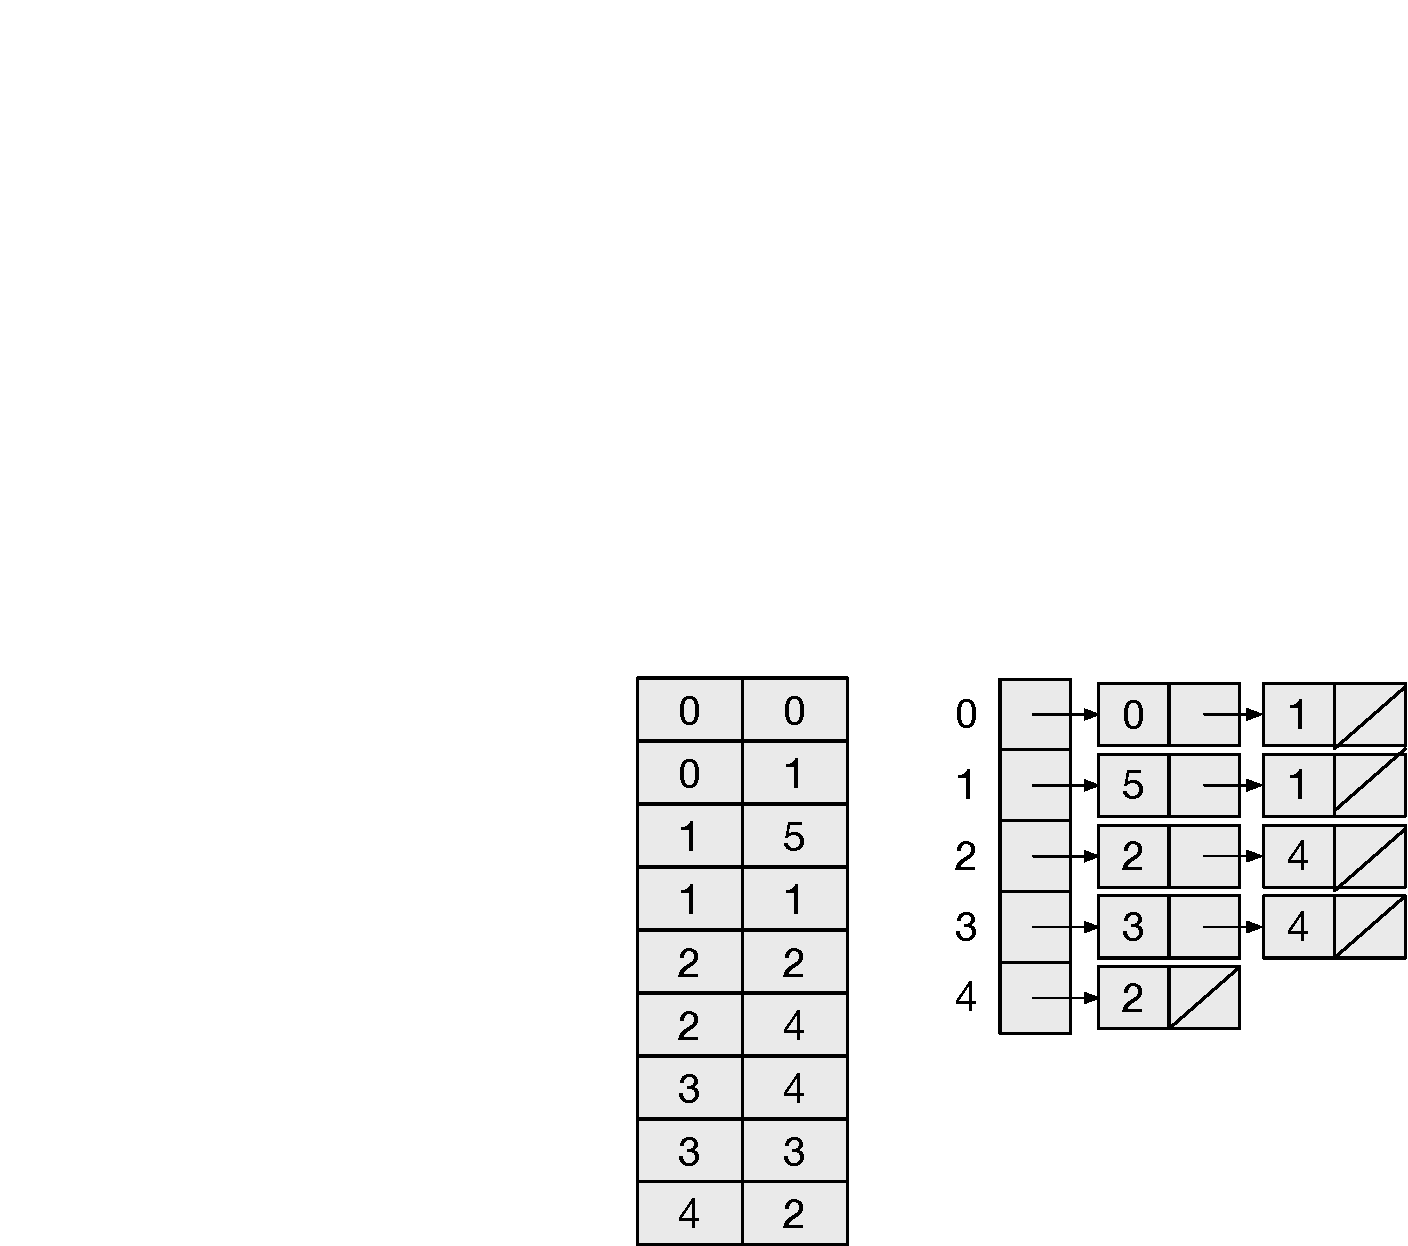
\includegraphics[width=0.825\linewidth]{figs/movie-actor-sparse-adjacency}
    \caption{\label{fig:actor-table}
    Coordinate and compressed sparse adjacency representations for movies with their starring actors.}
  \end{subfigure}
\hspace{1em}  
   \begin{subfigure}[t]{0.4\textwidth}
    \small
    \centering
    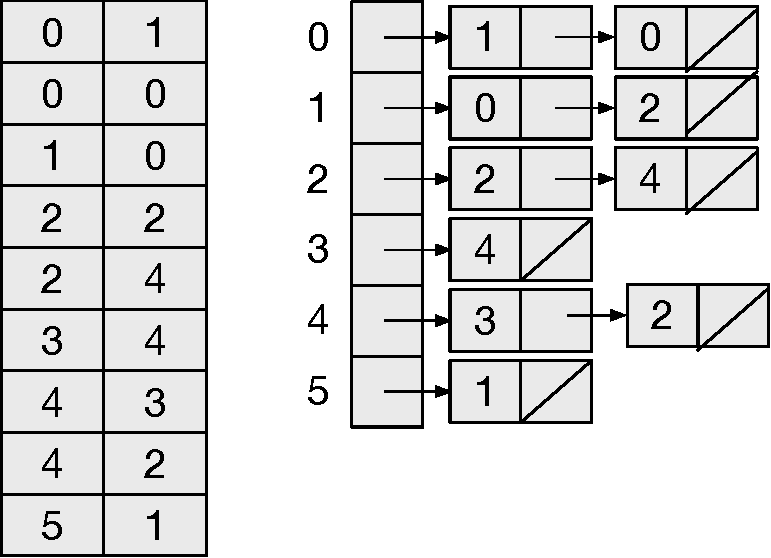
\includegraphics[width=0.825\linewidth]{figs/actor-movie-sparse-adjacency}
    \caption{\label{fig:movie-table}
    Coordinate and compressed sparse adjacency representations for actors and the movies they have appeared in.}
  \end{subfigure}
  \caption{Sparse adjacency representations (edge lists and adjacency lists) for IMDB actor and movie data.}
\end{figure}

We distinguish a structurally bipartite graph from simply a bipartite graph because the former applies separate enumerations to $U$ and $V$.  
In customary graph terminology, a \emph{bipartite} graph is one in which the vertices can be partitioned into two disjoint sets, such that all of the edges in the graph only connect vertices from one set to vertices of the other set.  However, although the vertices are partitioned, they are still taken from the same original vertex set $V$ and have a single enumeration.
Whether a graph can be partitioned in this way is a run-time property inherent to the graph itself (which can be discovered with an appropriate algorithm).  
This is not a natural way to model separate categories of entities, such as movies and actors, where entities are categorized completely independently of each other and it is therefore most appropriate to have independent enumerations for them.  
A structurally bipartite graph explicitly captures distinct vertex categories.
%

\section{Partitioned Graphs}

In contrast to structurally bipartite graphs, there are certainly cases
where one would want to maintain two categories of entities, or otherwise distinguish the vertices, from the same vertex set.  In that case, we would use a \emph{partitioned graph}, which we define as
$G = \{ V, E \}$, where the vertex set $V$ consists of non-overlapping subsets, i.e.,
$V = \{ V_0, V_1, \ldots \}$ which we enumerate as $V_0 = \{v_0, v_1, \ldots , v_{n0-1} \}$, 
$V_1 = \{ v_{n0}, \ldots , v_{n1-1} \}$ and so on.  Each $V_i$ is a \emph{partition} of $V$.
The total enumeration of $V$ is $V= \{ v_0, v_1, \ldots , v_{n-1} \}$.  Just as each $V_i$ is a partition of $V$, the enumeration of each $V_i$ is a partitioning of the enumeration of $V$.

The edge set $E$ still consists of edges $(v_i, v_j)$ (or $\{v_i, v_j\}$ where, in general, $v_i$ and $v_j$ may come from any partition.

We note that partitioned graphs are not restricted to two partitions---a partitioned graph can represent an arbitrary number of partitions, i.e., a \emph{multipartite} graph (a graph with multiple subsets of vertices such that edges only go between subsets).
While partitioned graphs can be used to model multipartite graphs, partitioned graphs are not necessarily multipartite; edges can comprise vertices within a partition as well as well as across partitions.


\section{From Data to Graph}

\subsection{Columnar Data}
Here we show how one might create an unlabeled edge list from a table of data stored in a CSV file.  The following loads a list of directed edges from a CSV file (the values in each row are assumed to be separated by whitespace)\footnote{We take a broad view of what a comma is.}.
The elements of the first column are considered to be the source vertices and the elements of
the second column are the destination vertices. If the edges also had properties, the third column
would contain the property values.  In this example, the edges are loaded into a vector of tuples, which meets the requirements of a (presumed) \lstinline{sparse_coordinate} concept.
\begin{lstlisting}[language=C++]
    auto sparse_coordinate edges = std::vector<std::tuple<vertex_id_t, vertex_id_t>;
    auto input = std::ifstream ("input.csv");
    vertex_id_t src, dst;
    while (input >> src >> dst) {
        edges.emplace_back (src, dst);
    }
\end{lstlisting}

Similarly, we could load a list of undirected edges from a CSV file into a 
\lstinline{sparse_coordinate} structure.  
Note that, as discussed above, the coordinate sparse adjacency matrix representation (aka an edge list), contains an entry $(i, j)$ as well as an entry $(j, i)$ for each undirected edge $\{ v_i, v_j \}$.  Hence, we add both \lstinline{(src, dst)} and  \lstinline{(dst, src)} to \lstinline{edges}.
\begin{lstlisting}[language=C++]
    auto sparse_coordinate edges = std::vector<std::tuple<vertex_id_t, vertex_id_t, double> edges;
    auto input = std::ifstream ("input.csv");
    vertex_id_t src, dst;
    double val;
    while (input >> src >> dst >> val) {
        edges.emplace_back (src, dst, val);
        edges.emplace_back (dst, src, val);
    }
\end{lstlisting}

These examples are meant to be illustrative and not necessarily
comprehensive (nor efficient).
There are, of course, many ways to define containers that meet the
requirements of the edge list concept and many ways to
create an edge list from columnar data.

\subsection{Converting an Edge List to an Adjacency List}

The following creates a compressed sparse representation (an adjacency list) from a coordinate sparse representation.  The adjacency list is represented as 
a \lstinline{std::vector<std::vector<vertex_id_t>>;}
\begin{lstlisting}[language=C++]
    auto sparse_coordinate edges = std::vector<std::tuple<vertex_id_t, vertex_id_t>;
    // Read the edges
    auto sparse_compressed adj_list = std::vector<std::vector<vertex_id_t>>;
    for (auto [src, dst] : edges) {
      if (src >= adj_list.size()) {
        adj_list.resize(src + 1);
      }
      adj_list[src].push_back (dst);
    }
\end{lstlisting}

We note that the \lstinline{sparse_coordinate} representation is agnostic as to whether it was originally created based on directed edges or undirected edges.  An optimization to the sparse coordinate representation would be to use a \emph{packed coordinate} representation, which would only maintain a single entry for each undirected edge.  In that case, we would need to have two complementary insertions into the adjacency list for each entry in the packed coordinate representation.

The following example illustrates the use of a packed coordinate format to construct an adjacency list with an edge property.
\begin{lstlisting}[language=C++]
    auto packed_sparse_coordinate edges = std::vector<std::tuple<vertex_id_t, vertex_id_t, double>>;
    // Read the edges
    auto compressed_sparse adj_list = std::vector<std::vector<std::tuple<vertex_id_t, double>>>(edges.num_vertices();
    for (auto [src, dst, val] : edges) {
      adj_list[src].push_back (dst, val);
      adj_list[dst].push_back (src, val);
    }
 \end{lstlisting}

% \andrew{We should have note that anything wrapped in a graph adapter has a `num\_vertices`
% method (and other members).
% We should also provide a constructor for the adapted adjacency list that takes and
% edge list as argument.}


% The examples above basically cover what I intened here.  Though perhaps we should
% explain in some more detail about what the concepts do, what kinds of things meet
% concept requirements, what the graph adapter does, etc.
% \section{Implementations}
% But maybe we can just cover those things further down and forward reference to
% them from here.

% \subsection{Edge List: Array of Structs / Struct of Arrays}
% \andrew{Edges can be stored as tuples (or tuple like) basically in parallel arrays (like a ranges::zip).}
% \subsection{Vertices and Edges: Node Objects and Link Objects}
% \andrew{ala Stanford Graph Base (et al).}
% \subsection{Adjacency List: Container of Containers}
% \andrew{An adjacency list can be represented as a container of containers (e.g., std::vector<std::list>).  Talk about range of ranges when we talk about library interfaces, requirements, concepts.  Note here that the structure of an adjacency list does not capture directedness -- directedness is a run-time property.}


% These are definitely already covered in the examples above.
% \subsection{From Edge List to Adjacency List}
% \andrew{Scan edge list and insert edgest into adjacency list.  Adjacency list must support insertion.}
% \subsection{Edge List and Adjacency List: Compressed Edge List}
% \andrew{Using a sort and group-by (or a sort, a run-length encoding, and a scan), we can compactify the edge-list reprentation and at the same time obtain an adjacency-list representation -- one that is memory and compute efficient.  Best of both worlds.  Has same basic structural principles as CSR / CSC matrices in linear algebra -- but much more general.}

\appendix

\subsection*{Problematic Terminology}
\label{sec:ambiguity}

Here we show how graph terminology in practical use is often ambiguous (and why we were so painstaking in our definitions).
The definitions of graph and adjacency list from \emph{The Handbook of Graph Theory, Second Edition} is a typical
example:\footnote{
Although we take this example of ambiguity
from the \emph{Handbook}, in general the \emph{Handbook} is a rigorous and extensive collection of
important theoretical results in graph theory.  We borrow from its formatting conventions here.
}
\begin{quote}
  \textbf{D1:} A directed graph or digraph $G = (V,E)$ consists of a finite, nonempty set of vertices $V$ and a set of edges $E$.
Each edge is an ordered pair $(v,w)$ of vertices.
\\[\medskipamount]
\textbf{E1:} A line drawing of a graph G = (V, E) is shown in Figure 1.1.1 [omitted, ed.]. It has vertex-set V = {u,v,w,x} and
edge-set E = {a,b,c,d,e,f}.
\\[\medskipamount]
\textbf{D9:} An adjacency list representation for a graph or digraph $G = (V, E)$ is an array $L$ of $|V|$ lists, one for each
vertex in $V$. For each vertex $i$, there is a pointer $L_i$ to a linked list containing all vertices $j$ adjacent to $i$.
\end{quote}
The ambiguity occurs between \textbf{D1}/\textbf{E1} and \textbf{D9}.

In \textbf{D1}, a vertex $v \in V$ is an element of unspecified type and in \textbf{E1} a particular case is given in $E1$ where
each vertex is a letter.  Indeed, in the literature, it is common to identify vertices in $V$ with domain entities that the graph
is modeling (``a vertex is a person'').  These are (literally) textbook definitions, and no one would bat an eye in reading them.

But if we look critically at \textbf{D9}, what is meant by ``vertex'' is completely ambiguous.  The adjacency list
in \textbf{D9} is representing graph $G=\{ V, E\}$, that is, by \textbf{D1}, a vertex is a member of $V$ and its type is
unspecified.  However, \textbf{D9} also uses the term ``vertex'' to refer to indices -- ``vertex'' $i$ indexes $L_i$, the linked list   
$L_i$ stores ``vertices'' -- yet, it is index values, not vertices that are being stored.  Beyond ``vertex,'' many other terms are
 ambiguously used when referring to graphs.  Perhaps the most egregious ambiguity is the term ``graph'' itself -- which is used to 
refer to the graph $G=\{ V, E \}$, to the representation of a graph, or even to the entities being modeled by the graph.

A more careful distinction needs to be made between a graph and its representation -- and between the abstractions associated with
a graph and the abstractions associated with the representation of a graph.  We can't use the same term (e.g., ``vertex'') to mean
two different things.
